\subsection{Generazione Immagini Corrotte}
\textbf{Obiettivo:}
Degradare le immagini applicando, mediante le funzioni riportate \\lla cella precedente,  l'operatore di blur con parametri
\begin{itemize}
    \item{$\sigma=0.5$ dimensione $5\times 5$}
    \item{$\sigma=1$ dimensione $7\times 7$}
    \item{$\sigma=1.3$ dimensione $9\times 9$}
\end{itemize}
ed aggiunge rumore gaussiano con deviazione standard (0, 0.05)

\begin{figure}[H]
    \centering
    \begin{minipage}[h]{\textwidth}
    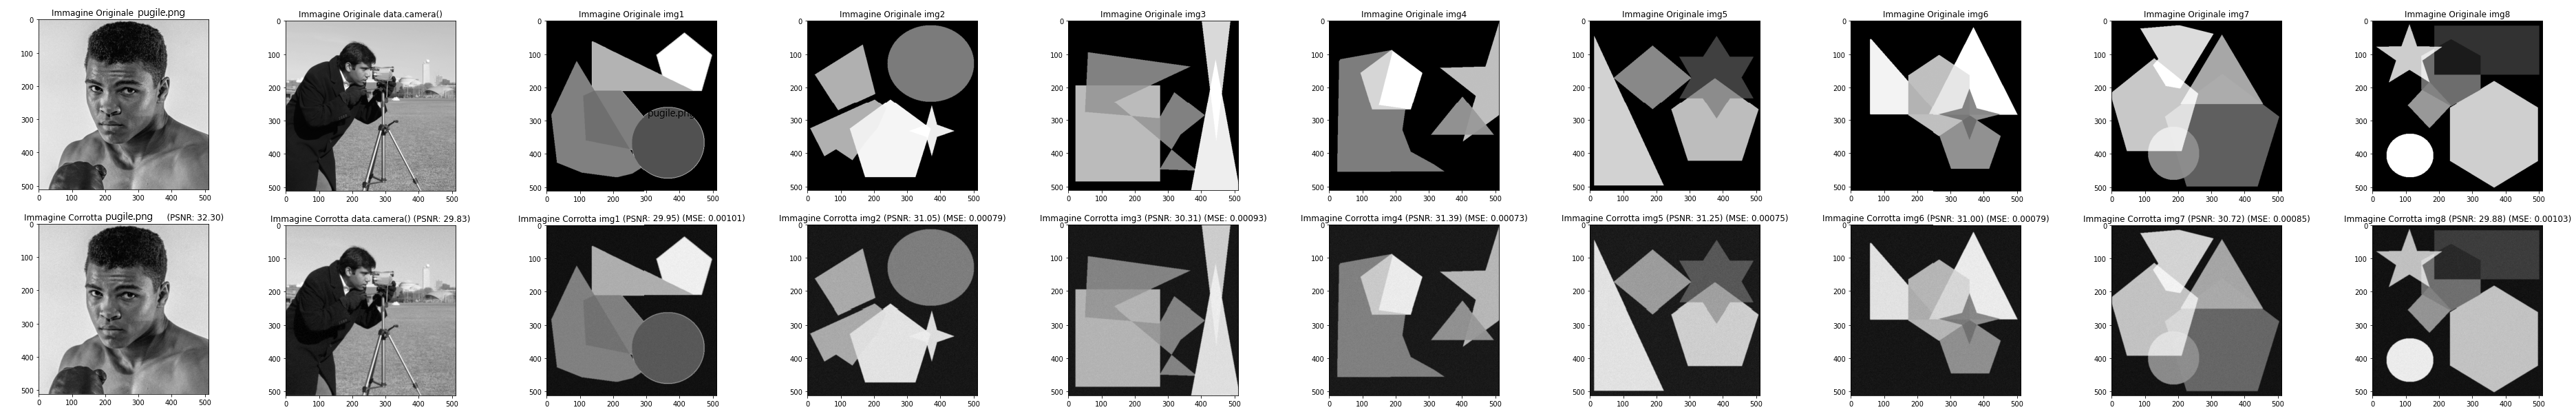
\includegraphics[width=\linewidth]{output/tabCorrotte/imgcorr1.png}\label{fig:imgcorrotte1}
    \end{minipage}
    \begin{minipage}[h]{\textwidth}
        \centering
        
        \begin{tabular}{|l c c c c r|}
            \hline
            \multicolumn{1}{|c}{\textbf{Nome Img}} & \multicolumn{1}{|c}{\textbf{DimKer}} & \multicolumn{1}{|c}{\textbf{Sigma}} & \multicolumn{1}{|c}{\textbf{Noise Dev}} & \multicolumn{1}{|c}{\textbf{PSNR}} & \multicolumn{1}{|c|}{\textbf{MSE}} \\ \hline
                img1.png & 5 & 0.5 & 0.02 & 29.9455 & 0.00101263 \\
                img2.png & 5 & 0.5 & 0.02 & 31.0498 & 0.000785276\\
                img3.png & 5 & 0.5 & 0.02 & 30.3053 & 0.000932107\\
                img4.png & 5 & 0.5 & 0.02 & 31.3947 & 0.000725313\\
                img5.png & 5 & 0.5 & 0.02 & 31.2456 & 0.00075065 \\
                img6.png & 5 & 0.5 & 0.02 & 30.9971 & 0.00079486 \\
                img7.png & 5 & 0.5 & 0.02 & 30.7187 & 0.000847478\\
                img8.png & 5 & 0.5 & 0.02 & 29.8802 & 0.00102797 \\
                pugile.png & 5 & 0.5 & 0.02 & 32.3195 & 0.0005862\\
                giornale.png & 5 & 0.5 & 0.02 & 23.7827 & 0.00418534 \\ \hline
        \end{tabular}\label{tab:tabcorrotte1}
    \end{minipage}
    \captionlistentry[table]{Table corrotte}
    \captionsetup{labelformat=andtable}
    \caption{Immagini corrotte con $\sigma = 0.5$ dimensione $5 \times 5$ e noise=0.02}
\end{figure}

\begin{figure}[H]
    \centering
    \begin{minipage}[h]{\textwidth}
    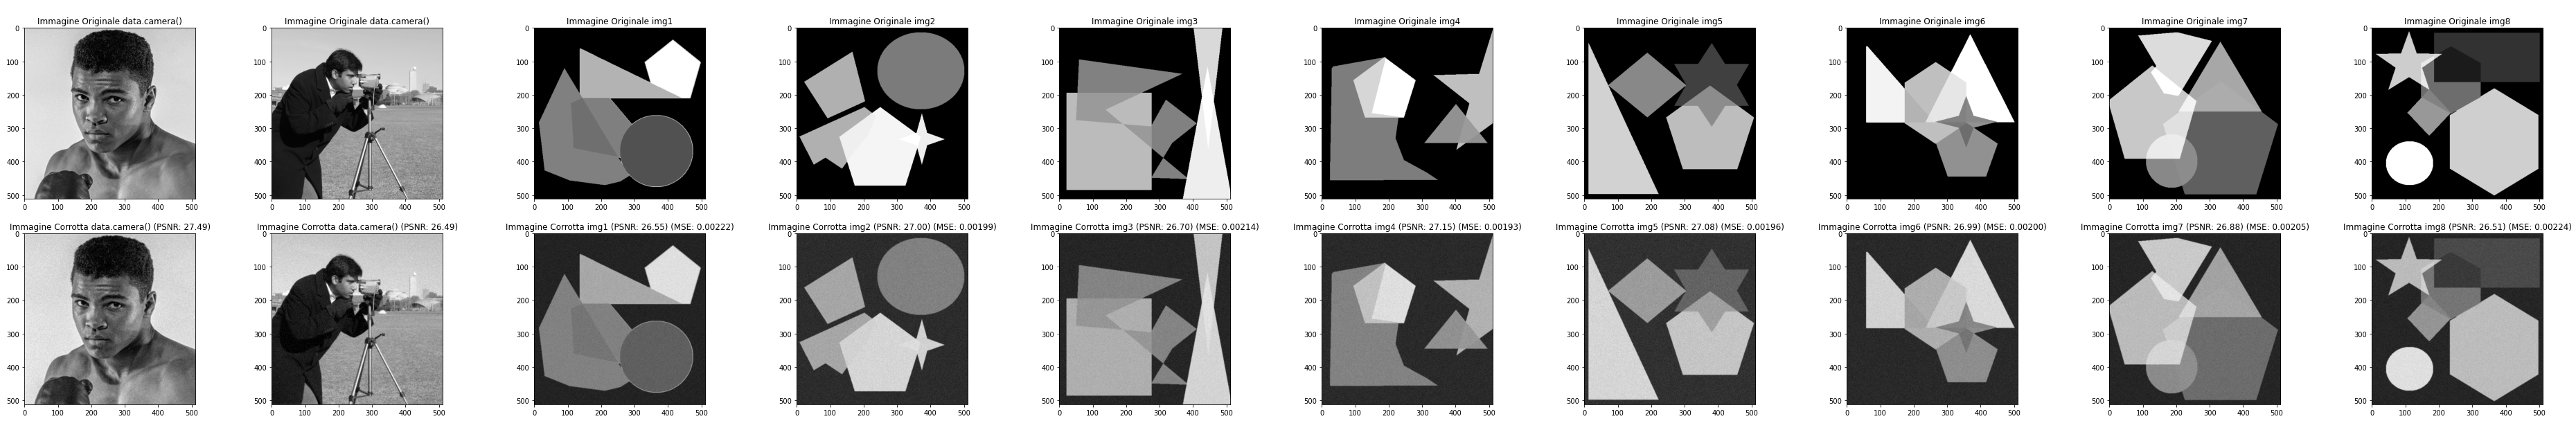
\includegraphics[width=\linewidth]{output/tabCorrotte/imgcorr2.png}\label{fig:imgcorrotte2}
    \end{minipage}
    \begin{minipage}[h]{\textwidth}
        \centering
        
        \begin{tabular}{|l c c c c r|}
            \hline
            \multicolumn{1}{|c}{\textbf{Nome Img}} & \multicolumn{1}{|c}{\textbf{DimKer}} & \multicolumn{1}{|c}{\textbf{Sigma}} & \multicolumn{1}{|c}{\textbf{Noise Dev}} & \multicolumn{1}{|c}{\textbf{PSNR}} & \multicolumn{1}{|c|}{\textbf{MSE}} \\ \hline
                img1.png & 5 & 0.5 & 0.04 & 26.5452 & 0.00221553 \\
                img2.png & 5 & 0.5 & 0.04 & 27.0007 & 0.00199492 \\
                img3.png & 5 & 0.5 & 0.04 & 26.6982 & 0.00213887 \\
                img4.png & 5 & 0.5 & 0.04 & 27.1549 & 0.00192537 \\
                img5.png & 5 & 0.5 & 0.04 & 27.0846 & 0.00195677 \\
                img6.png & 5 & 0.5 & 0.04 & 26.9876 & 0.00200098 \\
                img7.png & 5 & 0.5 & 0.04 & 26.8806 & 0.00205086 \\
                img8.png & 5 & 0.5 & 0.04 & 26.5063 & 0.00223545 \\
                pugile.png & 5 & 0.5 & 0.04 & 27.4667 & 0.0017919\\
                giornale.png & 5 & 0.5 & 0.04 & 22.7045 & 0.0053647 \\ \hline
            \end{tabular}\label{tab:tabcorrotte2}
        
        \end{minipage}
    \captionlistentry[table]{Table corrotte}
    \captionsetup{labelformat=andtable}
    \caption{Immagini corrotte con $\sigma = 0.5$ dimensione $5 \times 5$ e noise=0.04}
\end{figure}

\begin{figure}[H]
    \centering
    \begin{minipage}[h]{\textwidth}
    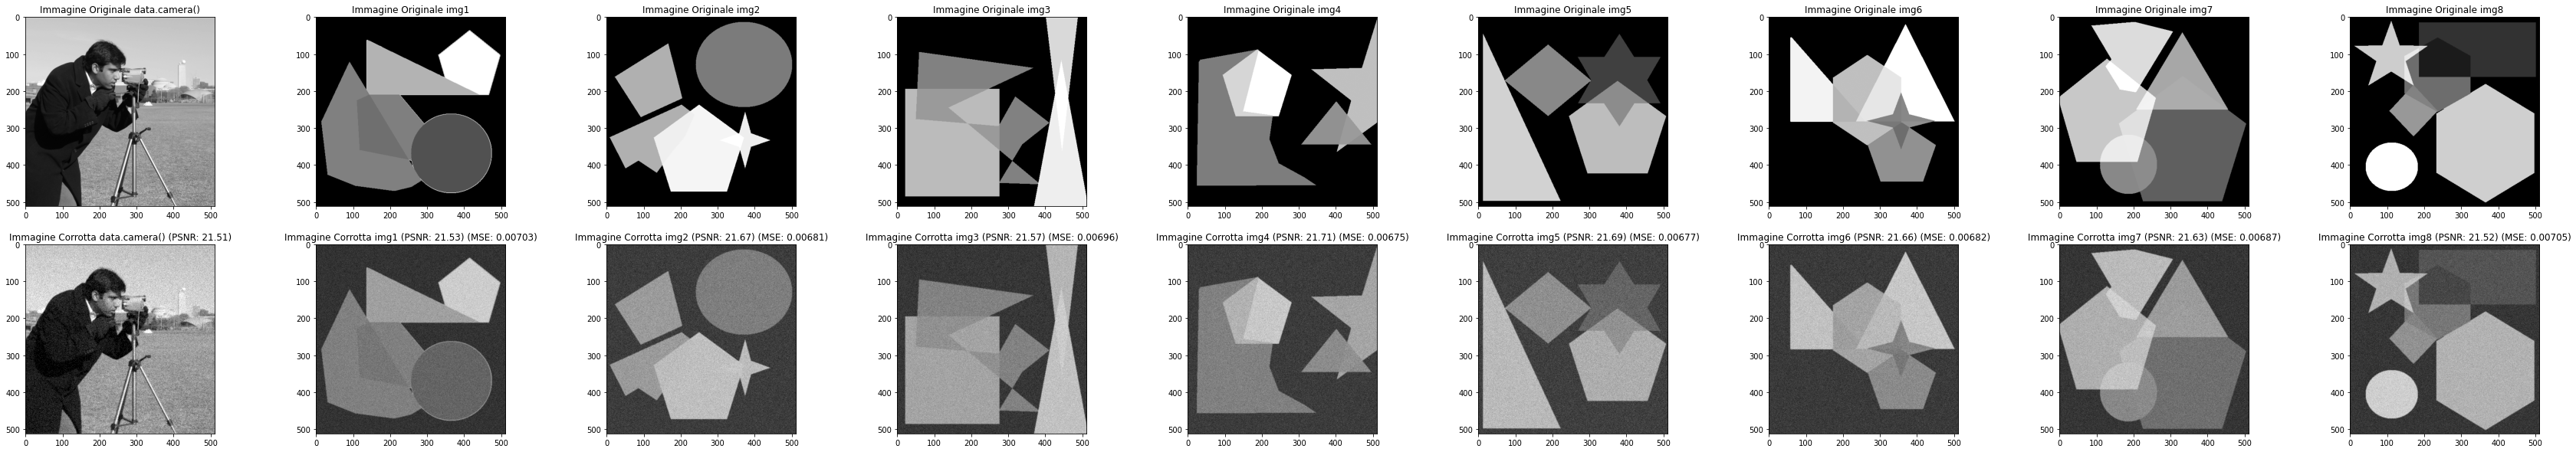
\includegraphics[width=\linewidth]{output/tabCorrotte/imgcorr3.png}\label{fig:imgcorrotte3}
    \end{minipage}
    \begin{minipage}[h]{\textwidth}
        \centering
        
        \begin{tabular}{|l c c c c r|}
            \hline
            \multicolumn{1}{|c}{\textbf{Nome Img}} & \multicolumn{1}{|c}{\textbf{DimKer}} & \multicolumn{1}{|c}{\textbf{Sigma}} & \multicolumn{1}{|c}{\textbf{Noise Dev}} & \multicolumn{1}{|c}{\textbf{PSNR}} & \multicolumn{1}{|c|}{\textbf{MSE}} \\ \hline
                img1.png & 5 & 0.5 & 0.08 & 21.5332 & 0.00702558 \\
                img2.png & 5 & 0.5 & 0.08 & 21.6702 & 0.00680731 \\
                img3.png & 5 & 0.5 & 0.08 & 21.5736 & 0.00696048 \\
                img4.png & 5 & 0.5 & 0.08 & 21.7089 & 0.00674704 \\
                img5.png & 5 & 0.5 & 0.08 & 21.6929 & 0.00677191 \\
                img6.png & 5 & 0.5 & 0.08 & 21.6626 & 0.00681931 \\
                img7.png & 5 & 0.5 & 0.08 & 21.633 & 0.00686601 \\
                img8.png & 5 & 0.5 & 0.08 & 21.519 & 0.00704858 \\
                pugile.png & 5 & 0.5 & 0.08 & 21.7986 & 0.0066091\\
                giornale.png & 5 & 0.5 & 0.08 & 19.9035 & 0.0102246 \\ \hline
            \end{tabular}v\label{tab:tabcorrotte3}
        
        \end{minipage}
    \captionlistentry[table]{Table corrotte}
    \captionsetup{labelformat=andtable}
    \caption{Immagini corrotte con $\sigma = 0.5$ dimensione $5 \times 5$ e noise=0.08}
\end{figure}

\begin{figure}[H]
    \centering
    \begin{minipage}[h]{\textwidth}
    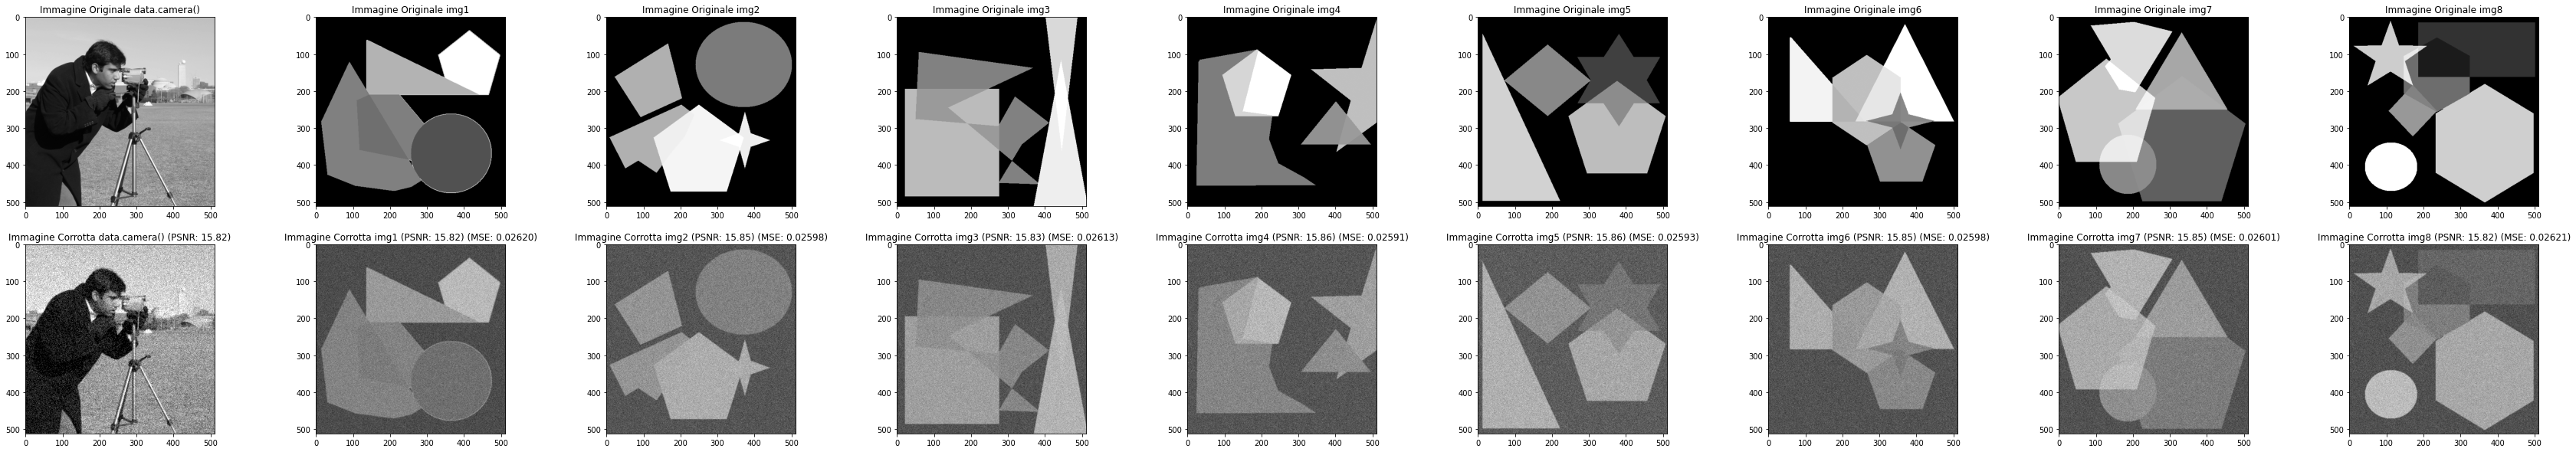
\includegraphics[width=\linewidth]{output/tabCorrotte/imgcorr4.png}\label{fig:imgcorrotte4}
    \end{minipage}
    \begin{minipage}[h]{\textwidth}
        \centering
        
        \begin{tabular}{|l c c c c r|}
            \hline
            \multicolumn{1}{|c}{\textbf{Nome Img}} & \multicolumn{1}{|c}{\textbf{DimKer}} & \multicolumn{1}{|c}{\textbf{Sigma}} & \multicolumn{1}{|c}{\textbf{Noise Dev}} & \multicolumn{1}{|c}{\textbf{PSNR}} & \multicolumn{1}{|c|}{\textbf{MSE}} \\ \hline
                img1.png & 5 & 0.5 & 0.16 & 15.8162 & 0.0262048 \\
                img2.png & 5 & 0.5 & 0.16 & 15.8543 & 0.025976 \\
                img3.png & 5 & 0.5 & 0.16 & 15.8278 & 0.0261347 \\
                img4.png & 5 & 0.5 & 0.16 & 15.8649 & 0.0259124 \\
                img5.png & 5 & 0.5 & 0.16 & 15.8618 & 0.0259313 \\
                img6.png & 5 & 0.5 & 0.16 & 15.8537 & 0.0259797 \\
                img7.png & 5 & 0.5 & 0.16 & 15.849 & 0.0260077 \\
                img8.png & 5 & 0.5 & 0.16 & 15.8161 & 0.0262051 \\
                pugile.png & 5 & 0.5 & 0.16 & 15.89 & 0.0257632 \\
                giornale.png & 5 & 0.5 & 0.16 & 15.3339 & 0.0292829 \\ \hline
            \end{tabular}\label{tab:tabcorrotte4}
        
        \end{minipage}
    \captionlistentry[table]{Table corrotte}
    \captionsetup{labelformat=andtable}
    \caption{Immagini corrotte con $\sigma = 0.5$ dimensione $5 \times 5$ e noise=0.16}
\end{figure}

\begin{figure}[H]
    \centering
    \begin{minipage}[h]{\textwidth}
    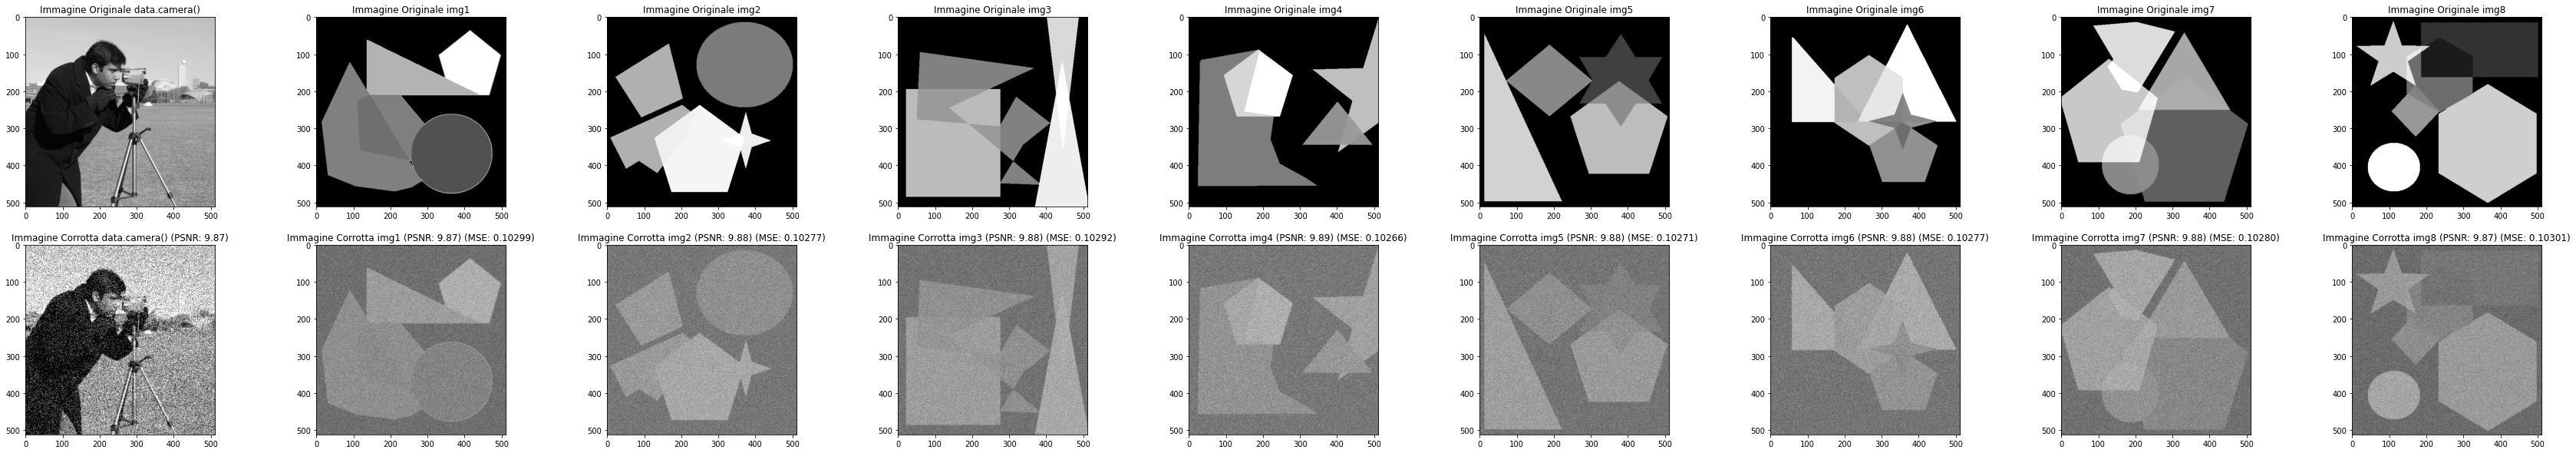
\includegraphics[width=\linewidth]{output/tabCorrotte/imgcorr5.png}\label{fig:imgcorrotte5}
    \end{minipage}
    \begin{minipage}[h]{\textwidth}
        \centering
        
        \begin{tabular}{|l c c c c r|}
            \hline
            \multicolumn{1}{|c}{\textbf{Nome Img}} & \multicolumn{1}{|c}{\textbf{DimKer}} & \multicolumn{1}{|c}{\textbf{Sigma}} & \multicolumn{1}{|c}{\textbf{Noise Dev}} & \multicolumn{1}{|c}{\textbf{PSNR}} & \multicolumn{1}{|c|}{\textbf{MSE}} \\ \hline
                img1.png & 5 & 0.5 & 0.32 & 9.8721 & 0.102989 \\                 
                img2.png & 5 & 0.5 & 0.32 & 9.88127 & 0.102772 \\ 
                img3.png & 5 & 0.5 & 0.32 & 9.87516 & 0.102916 \\
                img4.png & 5 & 0.5 & 0.32 & 9.8862 & 0.102655 \\                 
                img5.png & 5 & 0.5 & 0.32 & 9.88405 & 0.102706 \\ 
                img6.png & 5 & 0.5 & 0.32 & 9.88154 & 0.102765 \\
                img7.png & 5 & 0.5 & 0.32 & 9.88 & 0.102802 \\              
                img8.png & 5 & 0.5 & 0.32 & 9.87102 & 0.103014 \\ 
                pugile.png & 5 & 0.5 & 0.32 & 9.89115 & 0.102538 \\
                giornale.png & 5 & 0.5 & 0.32 & 9.73853 & 0.10620 \\ \hline
            \end{tabular}\label{tab:tabcorrotte5}  
        
        \end{minipage}
    \captionlistentry[table]{Table corrotte}
    \captionsetup{labelformat=andtable}
    \caption{Immagini corrotte con $\sigma = 0.5$ dimensione $5 \times 5$ e noise=0.32}
\end{figure}

\begin{figure}[H]
    \centering
    \begin{minipage}[h]{\textwidth}
    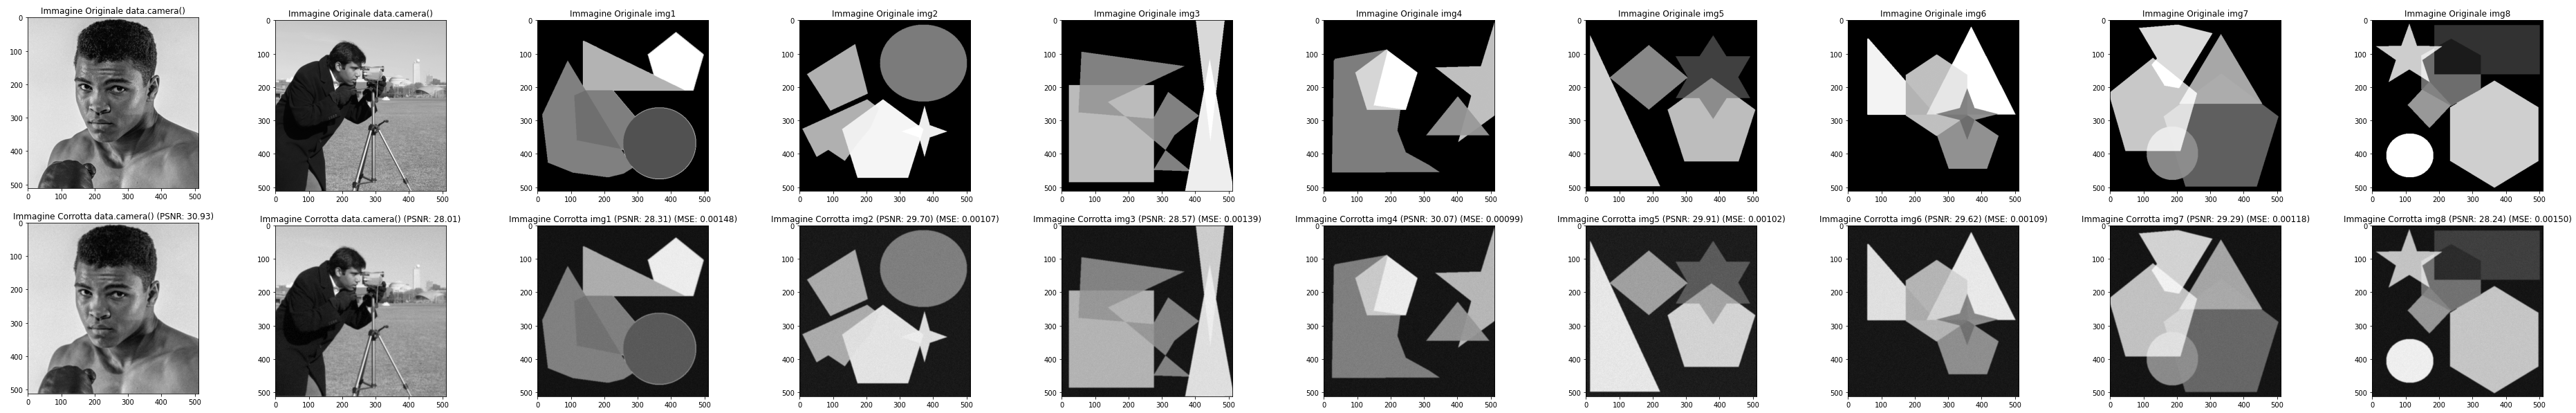
\includegraphics[width=\linewidth]{output/tabCorrotte/imgcorr6.png}\label{fig:imgcorrotte6}
    \end{minipage}
    \begin{minipage}[h]{\textwidth}
        \centering
        
        \begin{tabular}{|l c c c c r|}
            \hline
            \multicolumn{1}{|c}{\textbf{Nome Img}} & \multicolumn{1}{|c}{\textbf{DimKer}} & \multicolumn{1}{|c}{\textbf{Sigma}} & \multicolumn{1}{|c}{\textbf{Noise Dev}} & \multicolumn{1}{|c}{\textbf{PSNR}} & \multicolumn{1}{|c|}{\textbf{MSE}} \\ \hline
                img1.png & 7 & 1 & 0.02 & 28.3054 & 0.00147726 \\
                img2.png & 7 & 1 & 0.02 & 29.7038 & 0.00107057 \\
                img3.png & 7 & 1 & 0.02 & 28.5689 & 0.00139029 \\
                img4.png & 7 & 1 & 0.02 & 30.0656 & 0.000985011 \\
                img5.png & 7 & 1 & 0.02 & 29.9064 & 0.0010218 \\                 
                img6.png & 7 & 1 & 0.02 & 29.6228 & 0.00109074 \\ 
                img7.png & 7 & 1 & 0.02 & 29.2918 & 0.00117711 \\
                img8.png & 7 & 1 & 0.02 & 28.2434 & 0.00149851 \\
                pugile.png & 7 & 1 & 0.02 & 30.9284 & 0.000807527 \\
                giornale.png & 7 & 1 & 0.02 & 20.9194 & 0.0080921 \\ \hline
            \end{tabular}\label{tab:tabcorrotte6}
        
        \end{minipage}
    \captionlistentry[table]{Table corrotte}
    \captionsetup{labelformat=andtable}
    \caption{Immagini corrotte con $\sigma = 1$ dimensione $7 \times 7$ e noise=0.02}
\end{figure}

\begin{figure}[H]
    \centering
    \begin{minipage}[h]{\textwidth}
    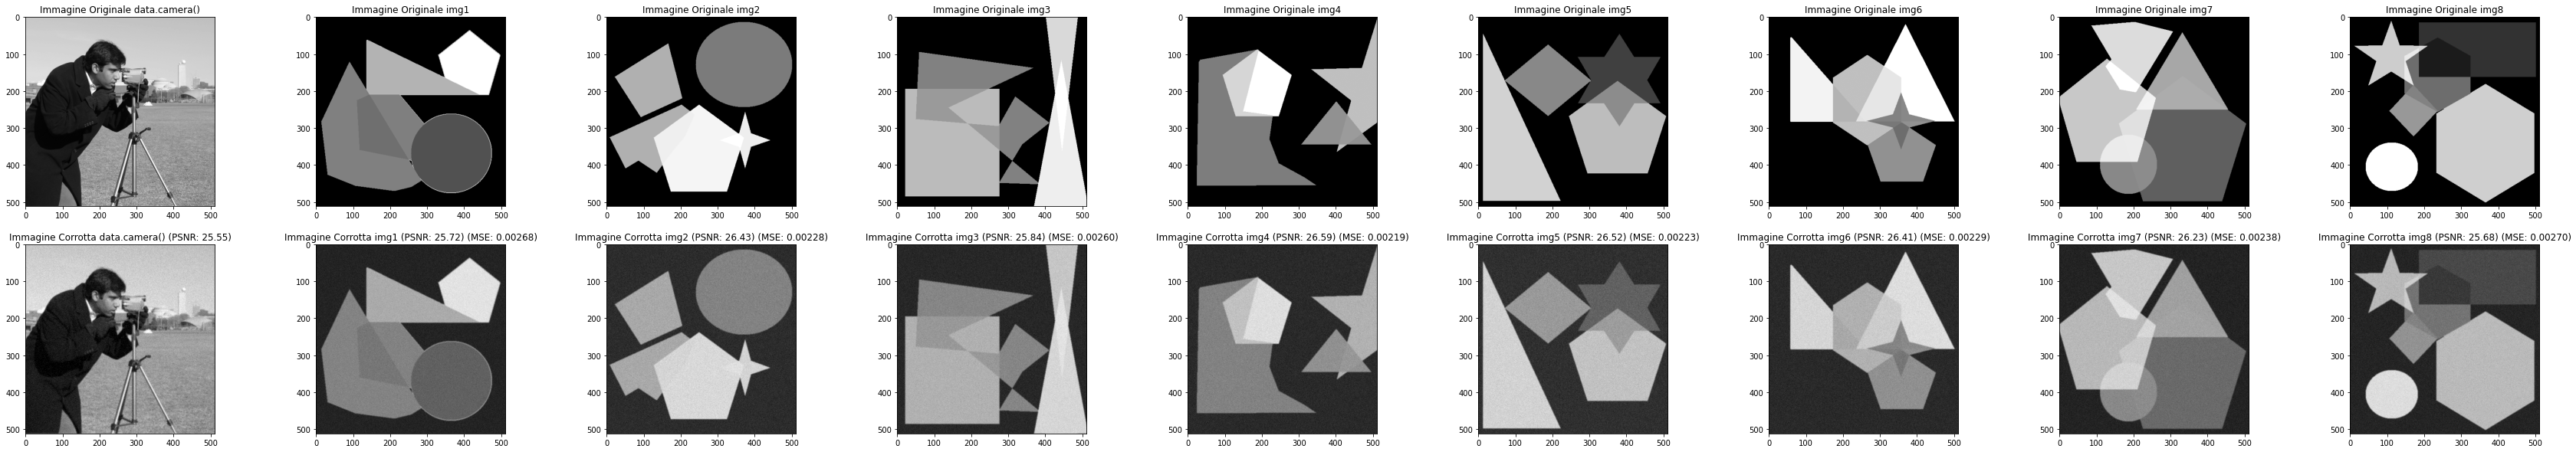
\includegraphics[width=\linewidth]{output/tabCorrotte/imgcorr7.png}\label{fig:imgcorrotte7}
    \end{minipage}
    \begin{minipage}[h]{\textwidth}
        \centering
        
        \begin{tabular}{|l c c c c r|}
            \hline
            \multicolumn{1}{|c}{\textbf{Nome Img}} & \multicolumn{1}{|c}{\textbf{DimKer}} & \multicolumn{1}{|c}{\textbf{Sigma}} & \multicolumn{1}{|c}{\textbf{Noise Dev}} & \multicolumn{1}{|c}{\textbf{PSNR}} & \multicolumn{1}{|c|}{\textbf{MSE}} \\ \hline
                img1.png & 7 & 1 & 0.04 & 25.7196 & 0.00267942 \\
                img2.png & 7 & 1 & 0.04 & 26.4282 & 0.00227604 \\
                img3.png & 7 & 1 & 0.04 & 25.8439 & 0.00260379 \\
                img4.png & 7 & 1 & 0.04 & 26.5898 & 0.0021929 \\                
                img5.png & 7 & 1 & 0.04 & 26.5209 & 0.00222797 \\ 
                img6.png & 7 & 1 & 0.04 & 26.4067 & 0.00228732 \\
                img7.png & 7 & 1 & 0.04 & 26.2277 & 0.00238357 \\
                img8.png & 7 & 1 & 0.04 & 25.6828 & 0.00270224 \\
                pugile.png & 7 & 1 & 0.04 & 26.9696 & 0.00200928 \\
                giornale.png & 7 & 1 & 0.04 & 20.3045 & 0.0093227\\ \hline
            \end{tabular}\label{tab:tabcorrotte7}
        
        \end{minipage}
    \captionlistentry[table]{Table corrotte}
    \captionsetup{labelformat=andtable}
    \caption{Immagini corrotte con $\sigma = 1$ dimensione $7 \times 7$ e noise=0.04}
\end{figure}

\begin{figure}[H]
    \centering
    \begin{minipage}[h]{\textwidth}
    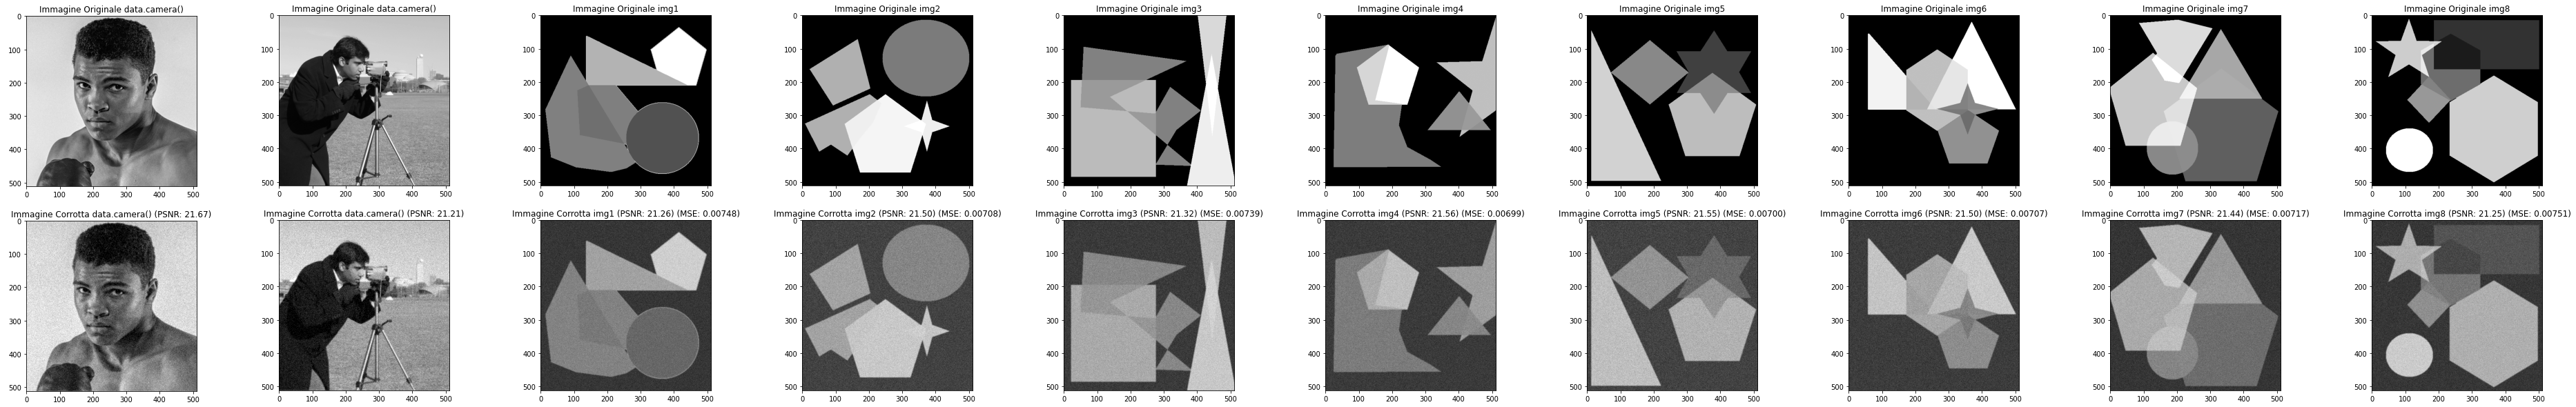
\includegraphics[width=\linewidth]{output/tabCorrotte/imgcorr8.png}\label{fig:imgcorrotte7x70.08}
    \end{minipage}
    \begin{minipage}[h]{\textwidth}
        \centering
        
        \begin{tabular}{|l c c c c r|}
            \hline
            \multicolumn{1}{|c}{\textbf{Nome Img}} & \multicolumn{1}{|c}{\textbf{DimKer}} & \multicolumn{1}{|c}{\textbf{Sigma}} & \multicolumn{1}{|c}{\textbf{Noise Dev}} & \multicolumn{1}{|c}{\textbf{PSNR}} & \multicolumn{1}{|c|}{\textbf{MSE}} \\ \hline
                img1.png & 7 & 1 & 0.08 & 21.2586 & 0.00748406 \\
                img2.png & 7 & 1 & 0.08 & 21.5025 & 0.00707543 \\
                img3.png & 7 & 1 & 0.08 & 21.3156 & 0.0073866 \\                 
                img4.png & 7 & 1 & 0.08 & 21.5582 & 0.00698523 \\
                img5.png & 7 & 1 & 0.08 & 21.5463 & 0.00700433 \\
                img6.png & 7 & 1 & 0.08 & 21.5043 & 0.00707252 \\
                img7.png & 7 & 1 & 0.08 & 21.4429 & 0.00717307 \\
                img8.png & 7 & 1 & 0.08 & 21.2464 & 0.00750518 \\
                pugile.png & 7 & 1 & 0.08 & 21.6733 & 0.00680245 \\
                giornale.png & 7 & 1 & 0.08 & 18.5164 & 0.0140722 \\ \hline
            \end{tabular}\label{tab:tabcorrotte7x70.08}
        \end{minipage}
    \captionlistentry[table]{Table corrotte}
    \captionsetup{labelformat=andtable}
    \caption{Immagini corrotte con $\sigma = 1$ dimensione $7 \times 7$ e noise=0.08}
\end{figure}

\begin{figure}[H]
    \centering
    \begin{minipage}[h]{\textwidth}
    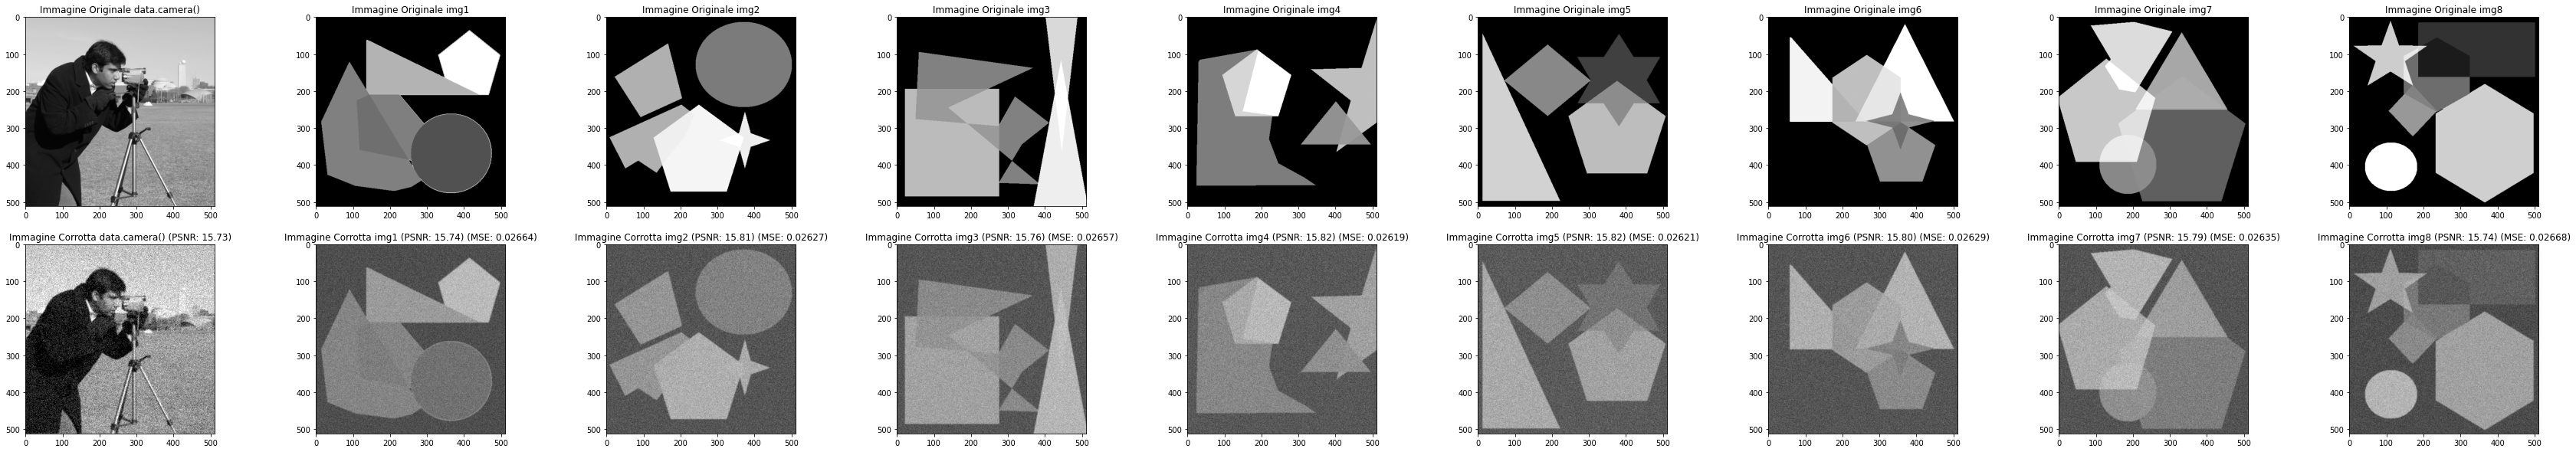
\includegraphics[width=\linewidth]{output/tabCorrotte/imgcorr9.png}\label{fig:imgcorrotte7x70.16}
    \end{minipage}
    \begin{minipage}[h]{\textwidth}
        \centering
        
        \begin{tabular}{|l c c c c r|}
            \hline
            \multicolumn{1}{|c}{\textbf{Nome Img}} & \multicolumn{1}{|c}{\textbf{DimKer}} & \multicolumn{1}{|c}{\textbf{Sigma}} & \multicolumn{1}{|c}{\textbf{Noise Dev}} & \multicolumn{1}{|c}{\textbf{PSNR}} & \multicolumn{1}{|c|}{\textbf{MSE}} \\ \hline
                img1.png & 7 & 1 & 0.16 & 15.7444 & 0.0266415 \\
                img2.png & 7 & 1 & 0.16 & 15.8054 & 0.0262698 \\ 
                img3.png & 7 & 1 & 0.16 & 15.7565 & 0.0265673 \\                 
                img4.png & 7 & 1 & 0.16 & 15.8194 & 0.0261856 \\
                img5.png & 7 & 1 & 0.16 & 15.8151 & 0.0262111 \\                 
                img6.png & 7 & 1 & 0.16 & 15.8029 & 0.0262853 \\
                img7.png & 7 & 1 & 0.16 & 15.7926 & 0.0263473 \\                 
                img8.png & 7 & 1 & 0.16 & 15.7385 & 0.0266776 \\
                pugile.png & 7 & 1 & 0.16 & 15.8496 & 0.0260039 \\
                giornale.png & 7 & 1 & 0.16 & 14.7736 & 0.0333153\\ \hline
            \end{tabular}\label{tab:tabcorrotte7x70.16}   
        
        \end{minipage}
    \captionlistentry[table]{Table corrotte}
    \captionsetup{labelformat=andtable}
    \caption{Immagini corrotte con $\sigma = 1$ dimensione $7 \times 7$ e noise=0.16}
\end{figure}

\begin{figure}[H]
    \centering
    \begin{minipage}[h]{\textwidth}
    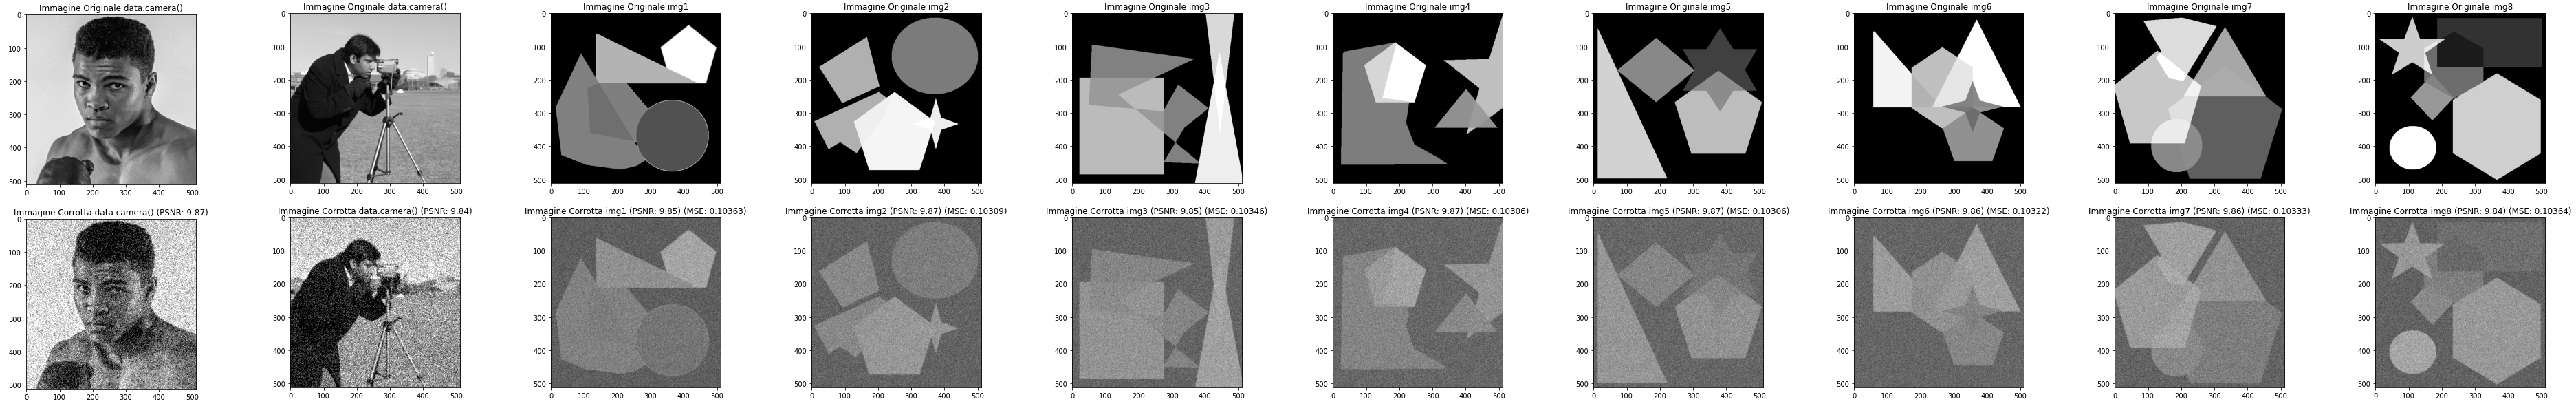
\includegraphics[width=\linewidth]{output/tabCorrotte/imgcorr10.png}\label{fig:imgcorrotte7x70.32}
    \end{minipage}
    \begin{minipage}[h]{\textwidth}
        \centering
        
        \begin{tabular}{|l c c c c r|}
            \hline
            \multicolumn{1}{|c}{\textbf{Nome Img}} & \multicolumn{1}{|c}{\textbf{DimKer}} & \multicolumn{1}{|c}{\textbf{Sigma}} & \multicolumn{1}{|c}{\textbf{Noise Dev}} & \multicolumn{1}{|c}{\textbf{PSNR}} & \multicolumn{1}{|c|}{\textbf{MSE}} \\ \hline
                img1.png & 7 & 1 & 0.32 & 9.84505 & 0.103632 \\ 
                img2.png & 7 & 1 & 0.32 & 9.86765 & 0.103094 \\
                img3.png & 7 & 1 & 0.32 & 9.85214 & 0.103463 \\
                img4.png & 7 & 1 & 0.32 & 9.86913 & 0.103059 \\
                img5.png & 7 & 1 & 0.32 & 9.869 & 0.103062 \\
                img6.png & 7 & 1 & 0.32 & 9.86252 & 0.103216 \\ 
                img7.png & 7 & 1 & 0.32 & 9.85775 & 0.10333 \\
                img8.png & 7 & 1 & 0.32 & 9.84472 & 0.10364 \\ 
                pugile.png & 7 & 1 & 0.32 & 9.87496 & 0.102921 \\
                giornale.png & 7 & 1 & 0.32 & 9.57992 & 0.110156 \\\hline
            \end{tabular}\label{tab:tabcorrotte7x70.32}   
        
        \end{minipage}
    \captionlistentry[table]{Table corrotte}
    \captionsetup{labelformat=andtable}
    \caption{Immagini corrotte con $\sigma = 1$ dimensione $7 \times 7$ e noise=0.32}
\end{figure}

\begin{figure}[H]
    \centering
    \begin{minipage}[h]{\textwidth}
    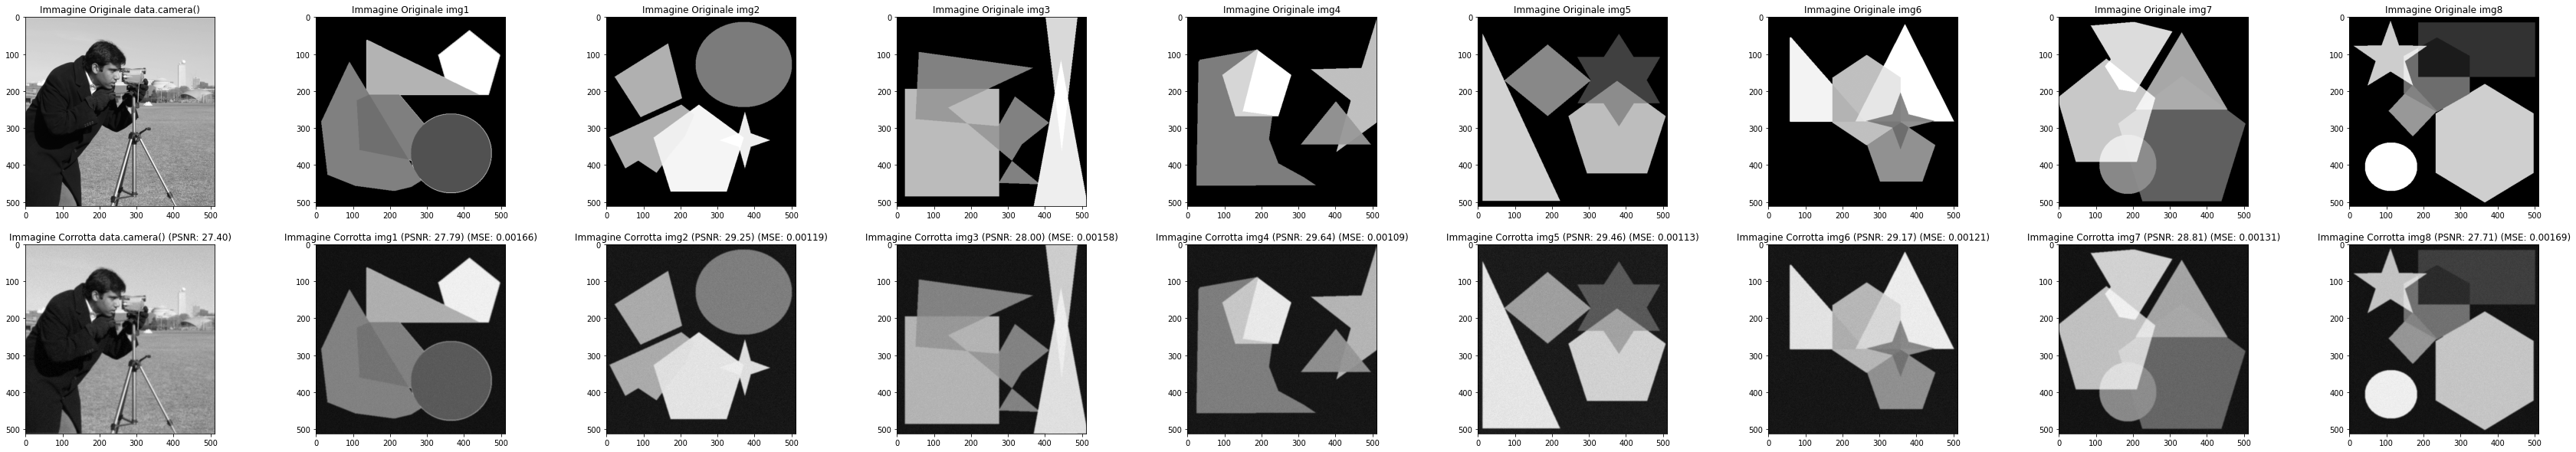
\includegraphics[width=\linewidth]{output/tabCorrotte/imgcorr11.png}\label{fig:imgcorrotte9x90.02}
    \end{minipage}
    \begin{minipage}[h]{\textwidth}
        \centering
        
        \begin{tabular}{|l c c c c r|}
            \hline
            \multicolumn{1}{|c}{\textbf{Nome Img}} & \multicolumn{1}{|c}{\textbf{DimKer}} & \multicolumn{1}{|c}{\textbf{Sigma}} & \multicolumn{1}{|c}{\textbf{Noise Dev}} & \multicolumn{1}{|c}{\textbf{PSNR}} & \multicolumn{1}{|c|}{\textbf{MSE}} \\ \hline
                img1.png & 9 & 1.3 & 0.02 & 27.7886 & 0.00166394 \\
                img2.png & 9 & 1.3 & 0.02 & 29.2539 & 0.00118745 \\
                img3.png & 9 & 1.3 & 0.02 & 28.0014 & 0.00158437 \\
                img4.png & 9 & 1.3 & 0.02 & 29.6382 & 0.00108688 \\
                img5.png & 9 & 1.3 & 0.02 & 29.4566 & 0.00113329 \\
                img6.png & 9 & 1.3 & 0.02 & 29.1727 & 0.00120986 \\
                img7.png & 9 & 1.3 & 0.02 & 28.8132 & 0.00131424 \\
                img8.png & 9 & 1.3 & 0.02 & 27.7142 & 0.00169269 \\
                pugile.png & 9 & 1.3 & 0.02 & 30.3576 & 0.0009209\\
                giornale.png & 9 & 1.3 & 0.02 & 20.0318 & 0.00992697 \\ \hline
            \end{tabular}\label{tab:tabcorrotte9x90.02}
        
        \end{minipage}
    \captionlistentry[table]{Table corrotte}
    \captionsetup{labelformat=andtable}
    \caption{Immagini corrotte con $\sigma = 1.3$ dimensione $9 \times 9$ e noise=0.02}
\end{figure}

\begin{figure}[H]
    \centering
    \begin{minipage}[h]{\textwidth}
    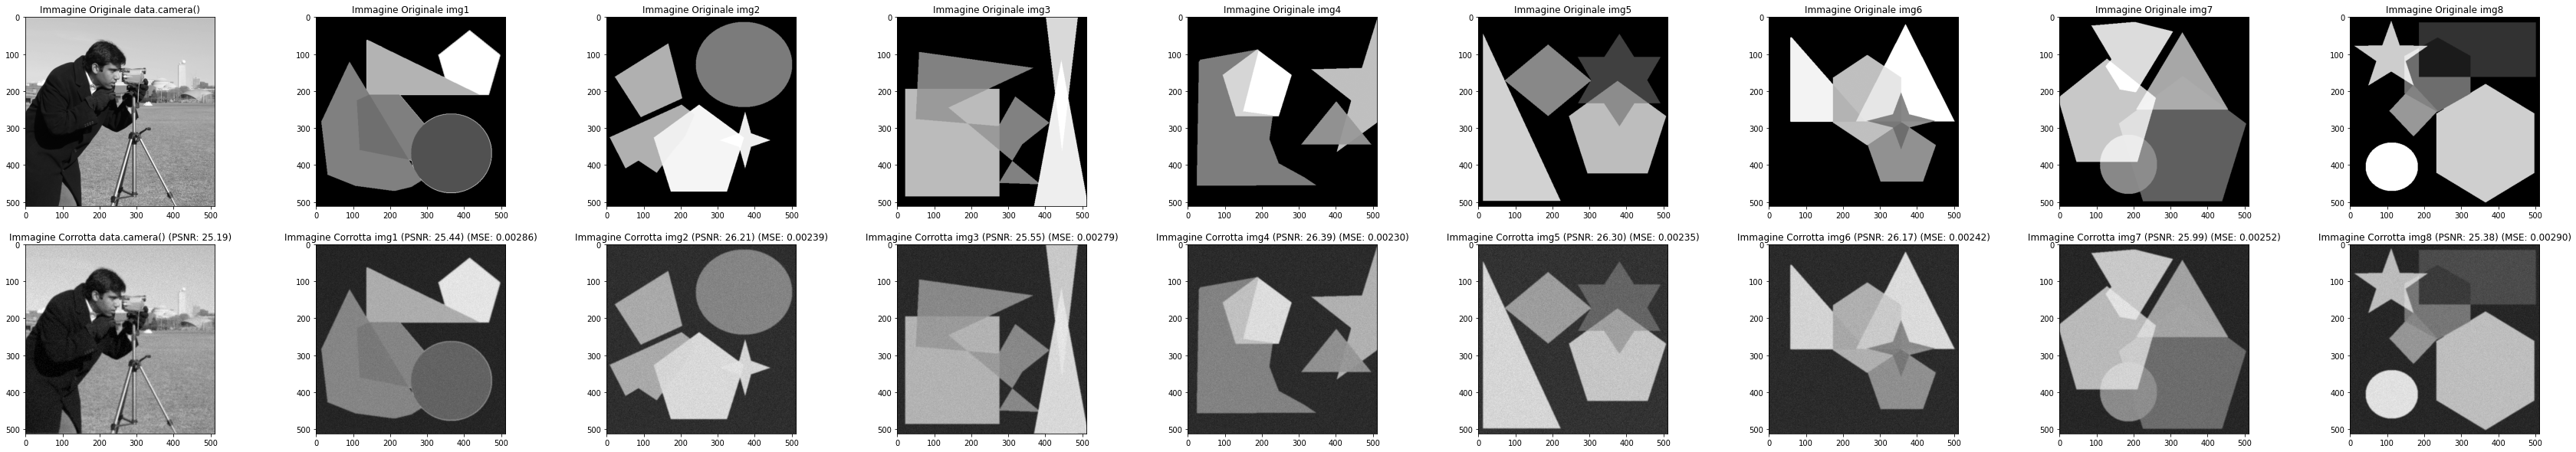
\includegraphics[width=\linewidth]{output/tabCorrotte/imgcorr12.png}\label{fig:imgcorrotte9x90.04}
    \end{minipage}
    \begin{minipage}[h]{\textwidth}
        \centering
        
        \begin{tabular}{|l c c c c r|}
            \hline
            \multicolumn{1}{|c}{\textbf{Nome Img}} & \multicolumn{1}{|c}{\textbf{DimKer}} & \multicolumn{1}{|c}{\textbf{Sigma}} & \multicolumn{1}{|c}{\textbf{Noise Dev}} & \multicolumn{1}{|c}{\textbf{PSNR}} & \multicolumn{1}{|c|}{\textbf{MSE}} \\ \hline
                img1.png & 9 & 1.3 & 0.04 & 25.4375 & 0.00285925 \\
                img2.png & 9 & 1.3 & 0.04 & 26.2124 & 0.00239202 \\
                img3.png & 9 & 1.3 & 0.04 & 25.5474 & 0.0027878 \\
                img4.png & 9 & 1.3 & 0.04 & 26.389 & 0.00229666 \\
                img5.png & 9 & 1.3 & 0.04 & 26.2972 & 0.00234571 \\
                img6.png & 9 & 1.3 & 0.04 & 26.1696 & 0.00241568 \\
                img7.png & 9 & 1.3 & 0.04 & 25.9907 & 0.00251728 \\
                img8.png & 9 & 1.3 & 0.04 & 25.3782 & 0.00289853 \\
                pugile.png & 9 & 1.3 & 0.04 & 26.7366 & 0.00212 \\
                giornale.png & 9 & 1.3 & 0.04 & 19.5402 & 0.0111168 \\ \hline
            \end{tabular}\label{tab:tabcorrotte9x90.04}
        
        \end{minipage}
    \captionlistentry[table]{Table corrotte}
    \captionsetup{labelformat=andtable}
    \caption{Immagini corrotte con $\sigma = 1.3$ dimensione $9 \times 9$ e noise=0.04}
\end{figure}


\begin{figure}[H]
    \centering
    \begin{minipage}[h]{\textwidth}
    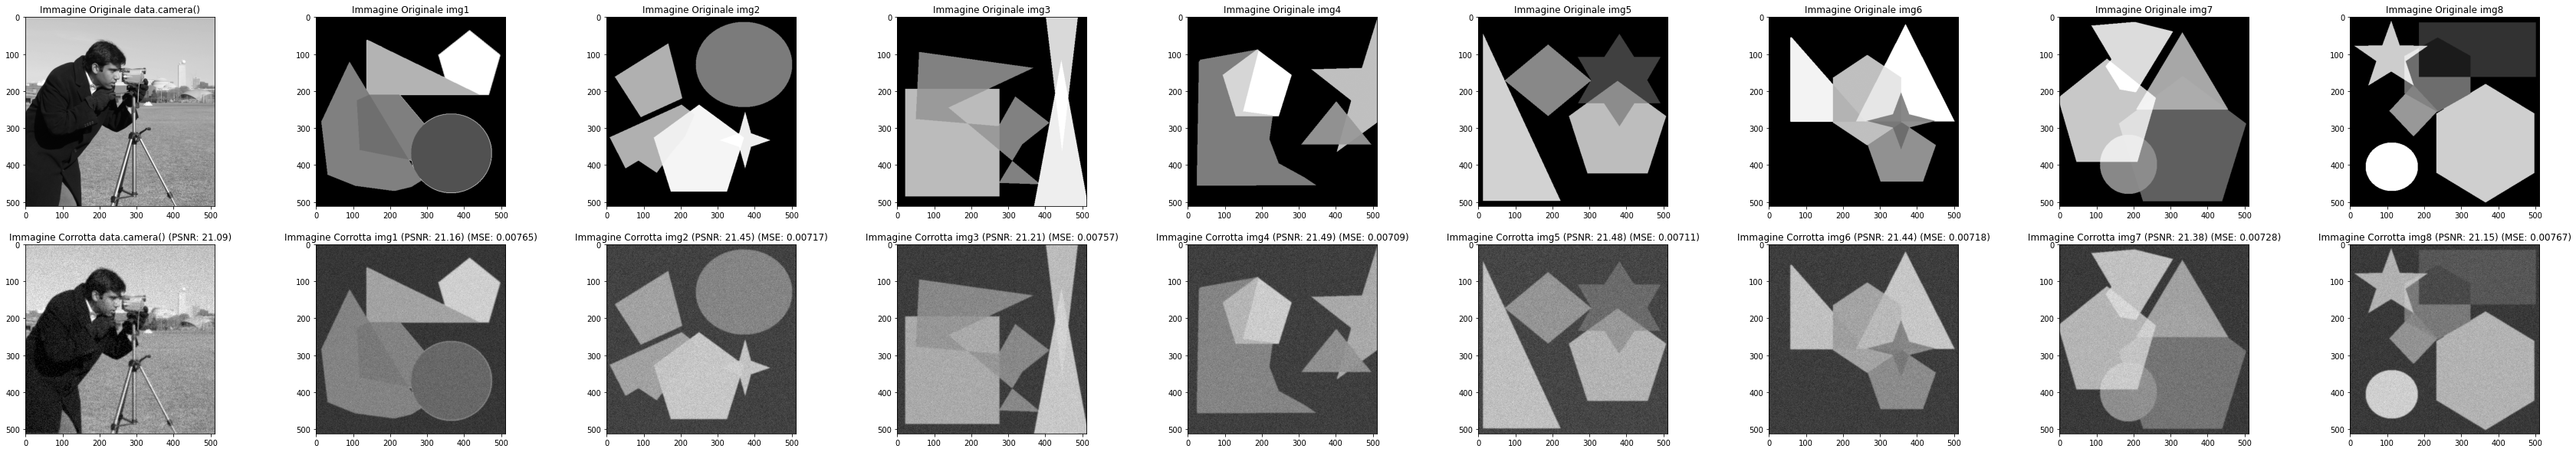
\includegraphics[width=\linewidth]{output/tabCorrotte/imgcorr13.png}\label{fig:imgcorrotte9x90.08}
    \end{minipage}
    \begin{minipage}[h]{\textwidth}
        \centering
        
        \begin{tabular}{|l c c c c r|}
            \hline
            \multicolumn{1}{|c}{\textbf{Nome Img}} & \multicolumn{1}{|c}{\textbf{DimKer}} & \multicolumn{1}{|c}{\textbf{Sigma}} & \multicolumn{1}{|c}{\textbf{Noise Dev}} & \multicolumn{1}{|c}{\textbf{PSNR}} & \multicolumn{1}{|c|}{\textbf{MSE}} \\ \hline
                img1.png & 9 & 1.3 & 0.08 & 21.1615 & 0.0076534 \\
                img2.png & 9 & 1.3 & 0.08 & 21.446 & 0.00716802 \\
                img3.png & 9 & 1.3 & 0.08 & 21.2099 & 0.00756858 \\
                img4.png & 9 & 1.3 & 0.08 & 21.4931 & 0.00709073 \\
                img5.png & 9 & 1.3 & 0.08 & 21.4791 & 0.0071136 \\
                img6.png & 9 & 1.3 & 0.08 & 21.436 & 0.0071845 \\
                img7.png & 9 & 1.3 & 0.08 & 21.3758 & 0.00728476 \\
                img8.png & 9 & 1.3 & 0.08 & 21.1529 & 0.00766845 \\
                pugile.png & 9 & 1.3 & 0.08 & 21.6072 & 0.0069068\\
                giornale.png & 9 & 1.3 & 0.08 & 17.9887 & 0.0158901 \\ \hline
            \end{tabular}\label{tab:tabcorrotte9x90.08}
        
        \end{minipage}
    \captionlistentry[table]{Table corrotte}
    \captionsetup{labelformat=andtable}
    \caption{Immagini corrotte con $\sigma = 1.3$ dimensione $9 \times 9$ e noise=0.08}
\end{figure}

\begin{figure}[H]
    \centering
    \begin{minipage}[h]{\textwidth}
    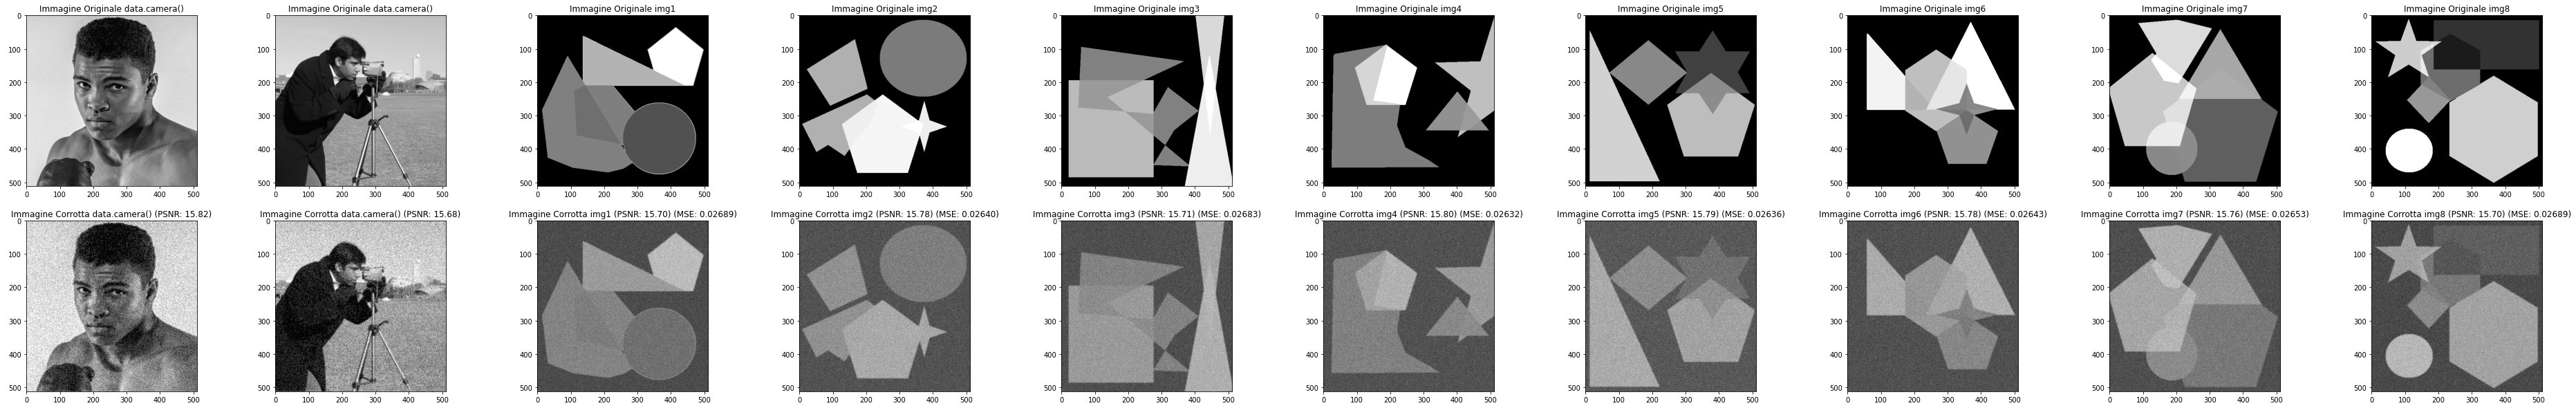
\includegraphics[width=\linewidth]{output/tabCorrotte/imgcorr14.png}\label{fig:imgcorrotte9x90.16}
    \end{minipage}
    \begin{minipage}[h]{\textwidth}
        \centering
        
        \begin{tabular}{|l c c c c r|}
            \hline
            \multicolumn{1}{|c}{\textbf{Nome Img}} & \multicolumn{1}{|c}{\textbf{DimKer}} & \multicolumn{1}{|c}{\textbf{Sigma}} & \multicolumn{1}{|c}{\textbf{Noise Dev}} & \multicolumn{1}{|c}{\textbf{PSNR}} & \multicolumn{1}{|c|}{\textbf{MSE}} \\ \hline
                img1.png & 9 & 1.3 & 0.16 & 15.7044 & 0.026888 \\
                img2.png & 9 & 1.3 & 0.16 & 15.7843 & 0.0263979 \\
                img3.png & 9 & 1.3 & 0.16 & 15.7146 & 0.0268251 \\
                img4.png & 9 & 1.3 & 0.16 & 15.7966 & 0.026323 \\
                img5.png & 9 & 1.3 & 0.16 & 15.7911 & 0.0263568 \\
                img6.png & 9 & 1.3 & 0.16 & 15.7794 & 0.0264277 \\
                img7.png & 9 & 1.3 & 0.16 & 15.7632 & 0.0265265 \\
                img8.png & 9 & 1.3 & 0.16 & 15.7044 & 0.0268884 \\
                pugile.png & 9 & 1.3 & 0.16 & 15.8334 & 0.0261013\\
                giornale.png & 9 & 1.3 & 0.16 & 14.5301 & 0.0352365 \\ \hline
            \end{tabular}\label{tab:tabcorrotte9x90.16}
        
        \end{minipage}
    \captionlistentry[table]{Table corrotte}
    \captionsetup{labelformat=andtable}
    \caption{Immagini corrotte con $\sigma = 1.3$ dimensione $9 \times 9$ e noise=0.16}
\end{figure}



\begin{figure}[H]
    \centering
    \begin{minipage}[h]{\textwidth}
    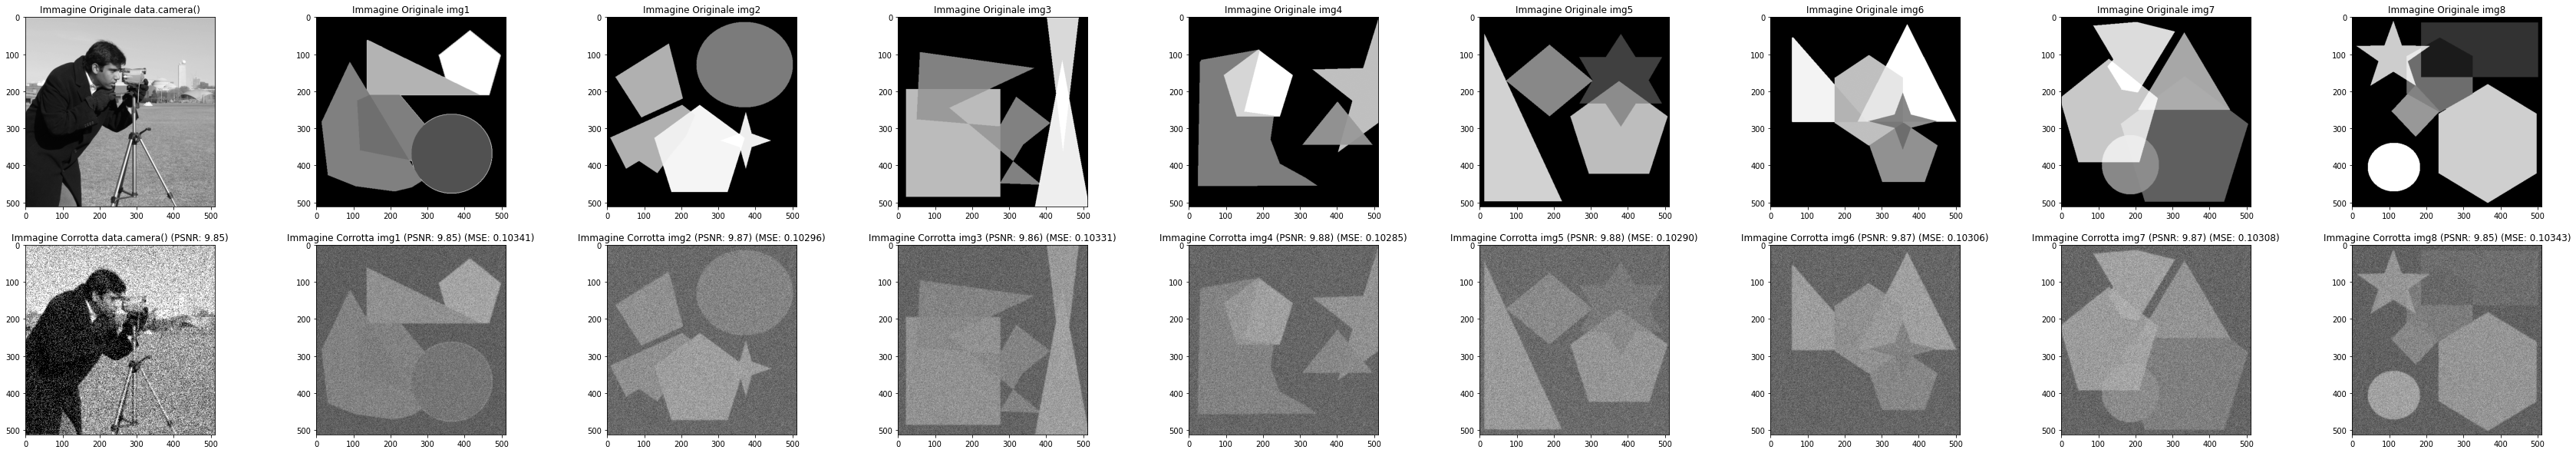
\includegraphics[width=\linewidth]{output/tabCorrotte/imgcorr15.png}\label{fig:imgcorrotte9x90.32}
    \end{minipage}
    \begin{minipage}[h]{\textwidth}
        \centering
        
        \begin{tabular}{|l c c c c r|}
            \hline
            \multicolumn{1}{|c}{\textbf{Nome Img}} & \multicolumn{1}{|c}{\textbf{DimKer}} & \multicolumn{1}{|c}{\textbf{Sigma}} & \multicolumn{1}{|c}{\textbf{Noise Dev}} & \multicolumn{1}{|c}{\textbf{PSNR}} & \multicolumn{1}{|c|}{\textbf{MSE}} \\ \hline
                img1.png & 9 & 1.3 & 0.32 & 9.85454 & 0.103406 \\
                img2.png & 9 & 1.3 & 0.32 & 9.87346 & 0.102957 \\
                img3.png & 9 & 1.3 & 0.32 & 9.85875 & 0.103306 \\
                img4.png & 9 & 1.3 & 0.32 & 9.87778 & 0.102854 \\
                img5.png & 9 & 1.3 & 0.32 & 9.87599 & 0.102897 \\
                img6.png & 9 & 1.3 & 0.32 & 9.86911 & 0.10306 \\ 
                img7.png & 9 & 1.3 & 0.32 & 9.8681 & 0.103084 \\ 
                img8.png & 9 & 1.3 & 0.32 & 9.85336 & 0.103434 \\
                pugile.png & 9 & 1.3 & 0.32 & 9.88385 & 0.10271 \\
                giornale.png & 9 & 1.3 & 0.32 & 9.52564 & 0.111541 \\ \hline
            \end{tabular}\label{tab:tabcorrotte9x90.32}
        
        \end{minipage}
    \captionlistentry[table]{Table corrotte}
    \captionsetup{labelformat=andtable}
    \caption{Immagini corrotte con $\sigma = 1.3$ dimensione $9 \times 9$ e noise=0.32}
\end{figure}

\begin{figure}[H]
    \centering
    \begin{minipage}[h]{0.58\textwidth}
    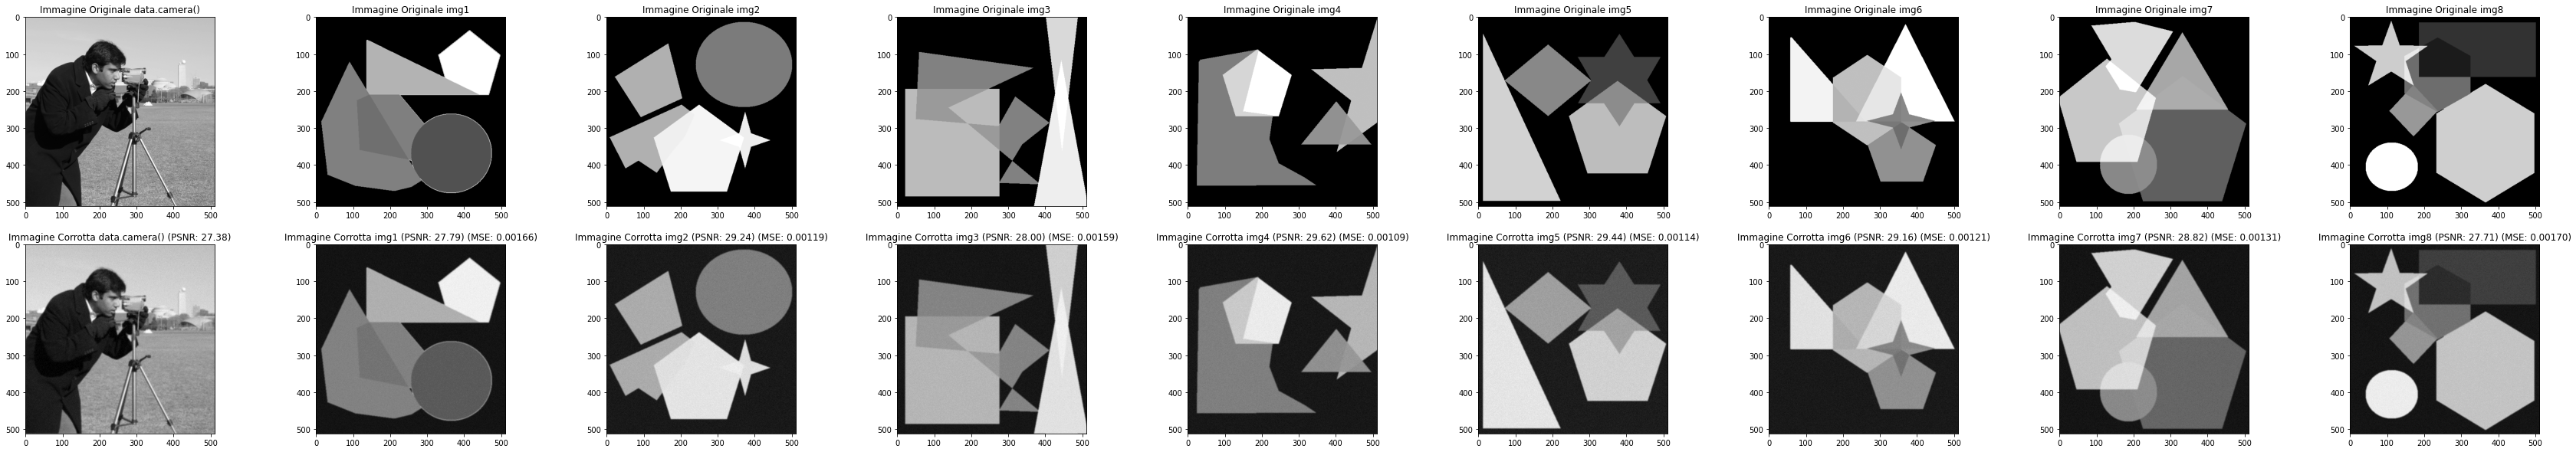
\includegraphics[width=\linewidth]{output/tabCorrotte/imgcorr0.png}\label{fig:imgcorrotteGEN}
    \end{minipage}%
    \begin{minipage}[h]{0.5\textwidth}
        \centering
        \begin{tabular}{|lr|}
            \hline
            \multicolumn{2}{|c|}{\textbf{Istanza del Problema}} \\ \hline
            Media PSNR           & 28.721034907424552           \\
            Media MSE            & 0.0013616018508439164        \\
            Dev. Std. PSNR       & 0.7263716130347668           \\
            Dev. Std. MSE        & 0.00032199072780323465       \\ \hline
            \end{tabular}
    \end{minipage}
    \captionlistentry[table]{Table corrotte}
    \captionsetup{labelformat=andtable}
    \caption{Immagini corrotte}
\end{figure}
